%% Supplementary material for the Artemis II seismo-acoustic paper.
%% Compile:  latexmk -pdf Artemis2supplement.tex
\documentclass[11pt]{article}
\usepackage[margin=2.2cm]{geometry}
\usepackage{graphicx}
\usepackage{siunitx}
\usepackage{booktabs}
\usepackage[font=small]{caption}
\graphicspath{{figures/}}
\renewcommand{\thefigure}{S\arabic{figure}}
\renewcommand{\thetable}{S\arabic{table}}
\setlength{\parindent}{0pt}

\title{Supplementary material for\\ ``The acoustic source of the Artemis~II launch: directivity, crackle and acoustic tracking from a dense seismo-acoustic network''}
\author{Glenn Thompson, Paul Bremner, Han Byul Woo, Sue Bilek}
\date{}

\begin{document}
\maketitle

Figures S1--S5 and Tables S1--S2 support the main text. They were produced by the notebooks in
\texttt{09\_artemis2\_paper} (numbers in brackets).

\begin{figure}[p]
  \centering
  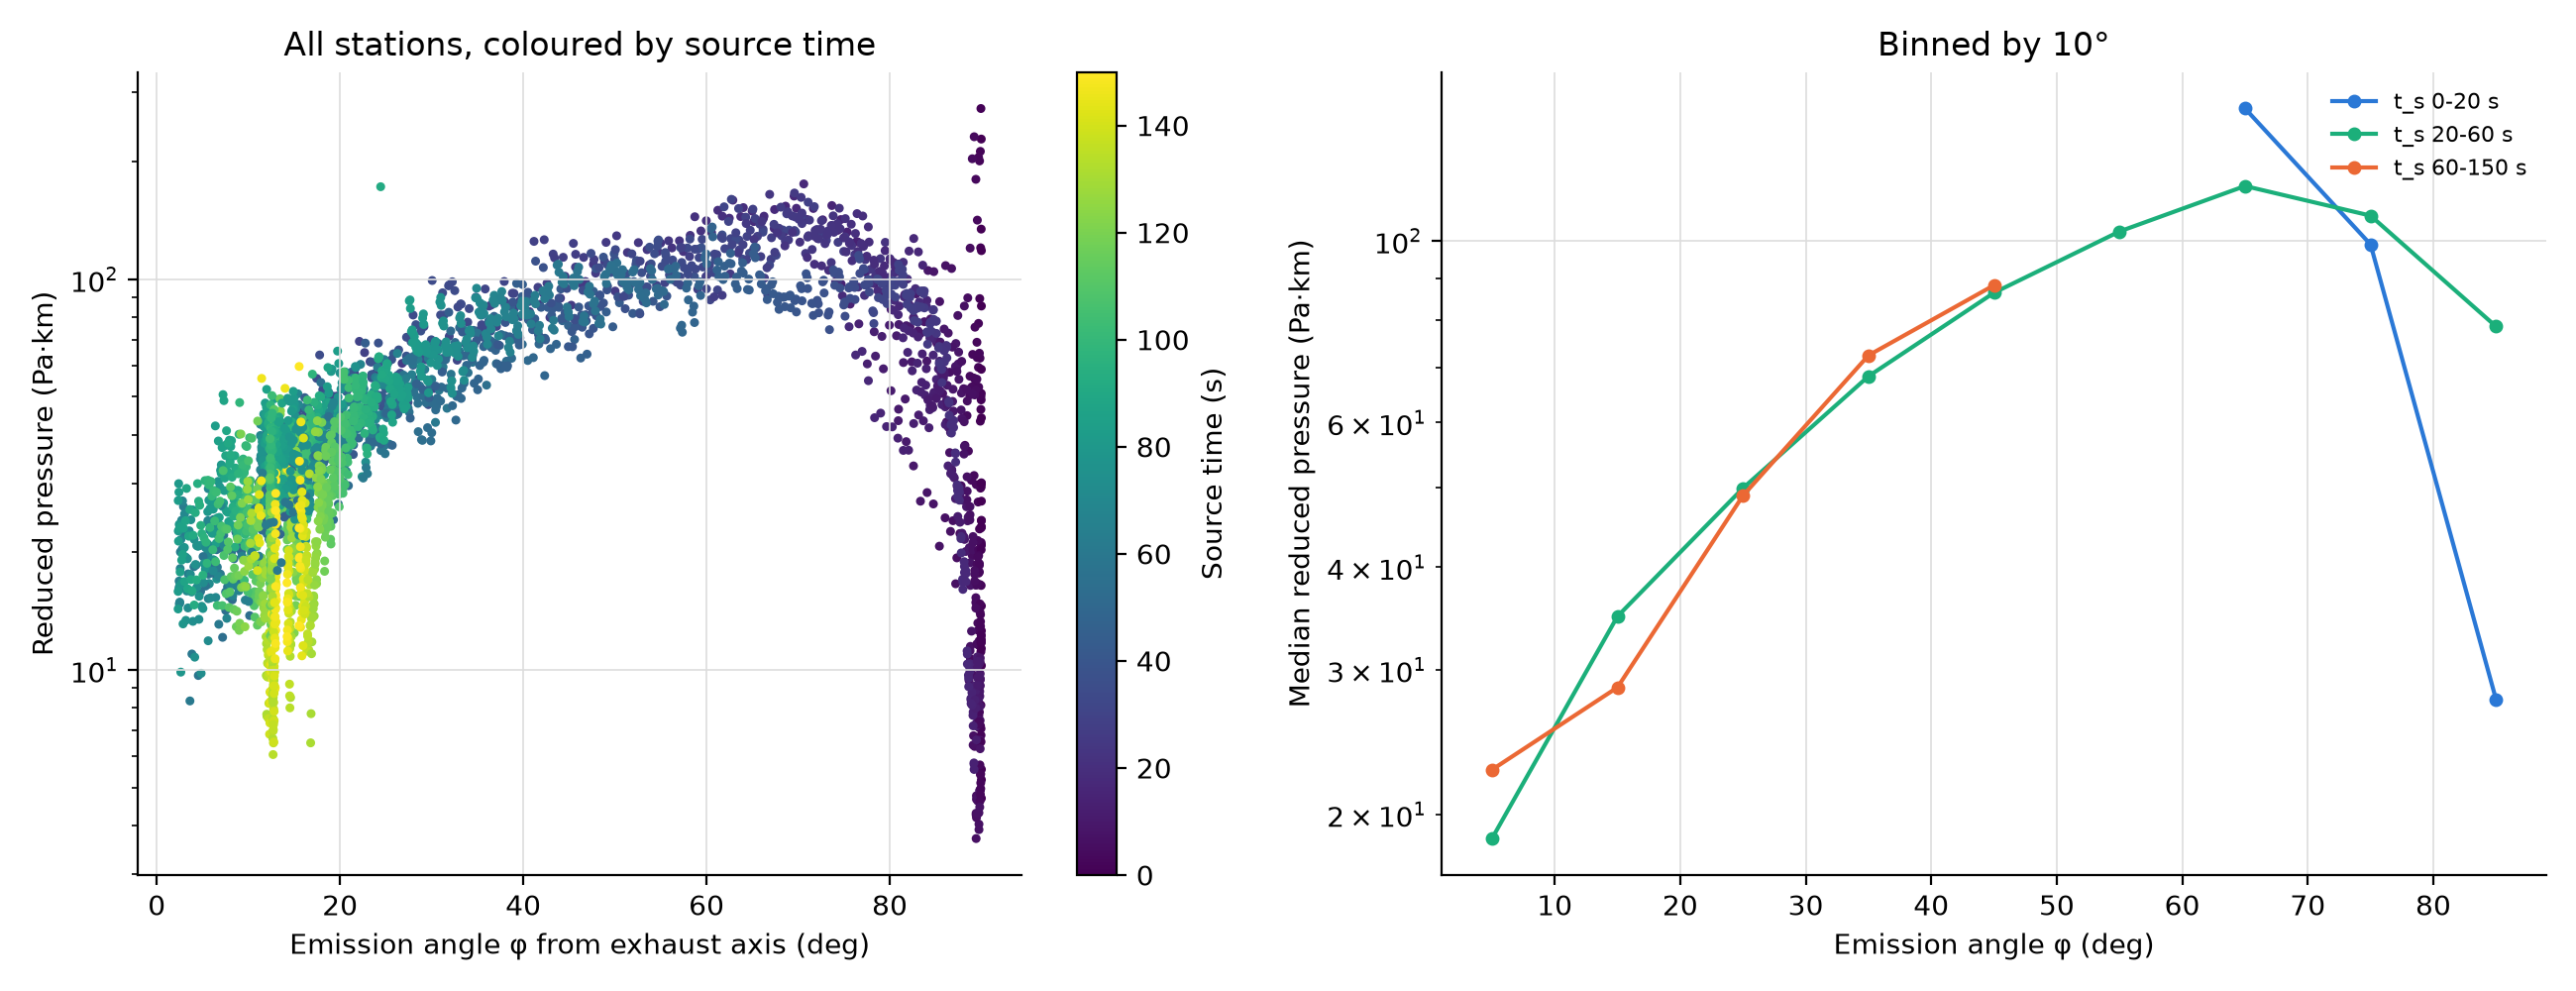
\includegraphics[width=\textwidth]{moving_source_directivity}
  \caption{Reduced pressure against emission angle $\phi$ from the
    exhaust axis. Left: all stations and source times, coloured by
    source time. Right: medians in 10$^{\circ}$ bins for three ranges
    of source time.}
  \label{fig:directivity}
\end{figure}


\begin{figure}[p]
  \centering
  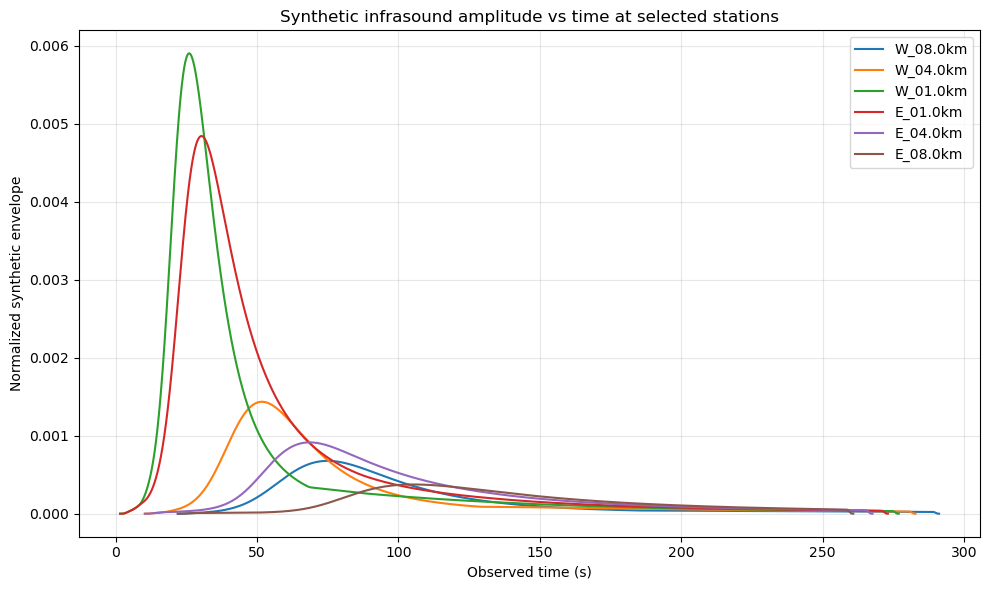
\includegraphics[width=\textwidth]{synthetic_envelopes}
  \caption{Synthetic infrasound envelopes at selected west (W) and east (E)
    virtual stations as a function of observed time [35], for the originally
    assumed directivity ($\phi_0 = 30^{\circ}$, $\sigma = 20^{\circ}$). At a
    given distance, west stations peak earlier and with higher amplitude than
    east stations.}
\end{figure}

\begin{figure}[p]
  \centering
  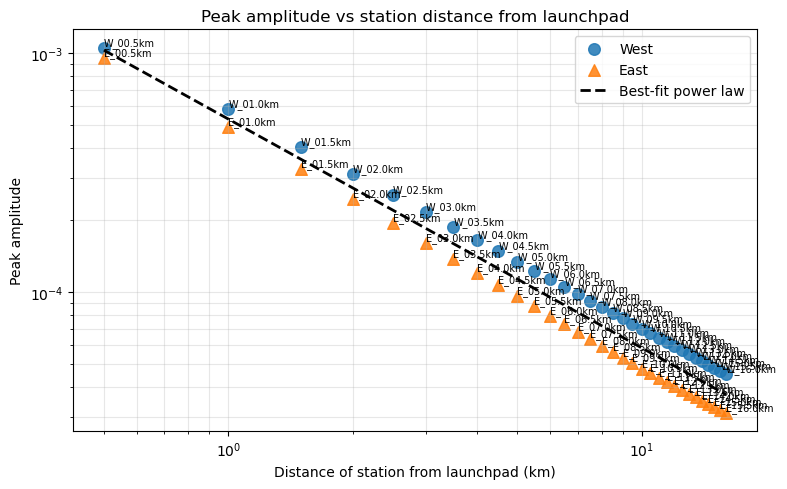
\includegraphics[width=0.8\textwidth]{synthetic_amplitude_vs_distance}
  \caption{Synthetic peak amplitude versus distance on idealized west (circles)
    and east (triangles) station lines for the originally assumed directivity
    (30$^{\circ}$, 20$^{\circ}$), with the best-fit power law (exponent
    $-0.96$) [35].}
\end{figure}

\begin{figure}[p]
  \centering
  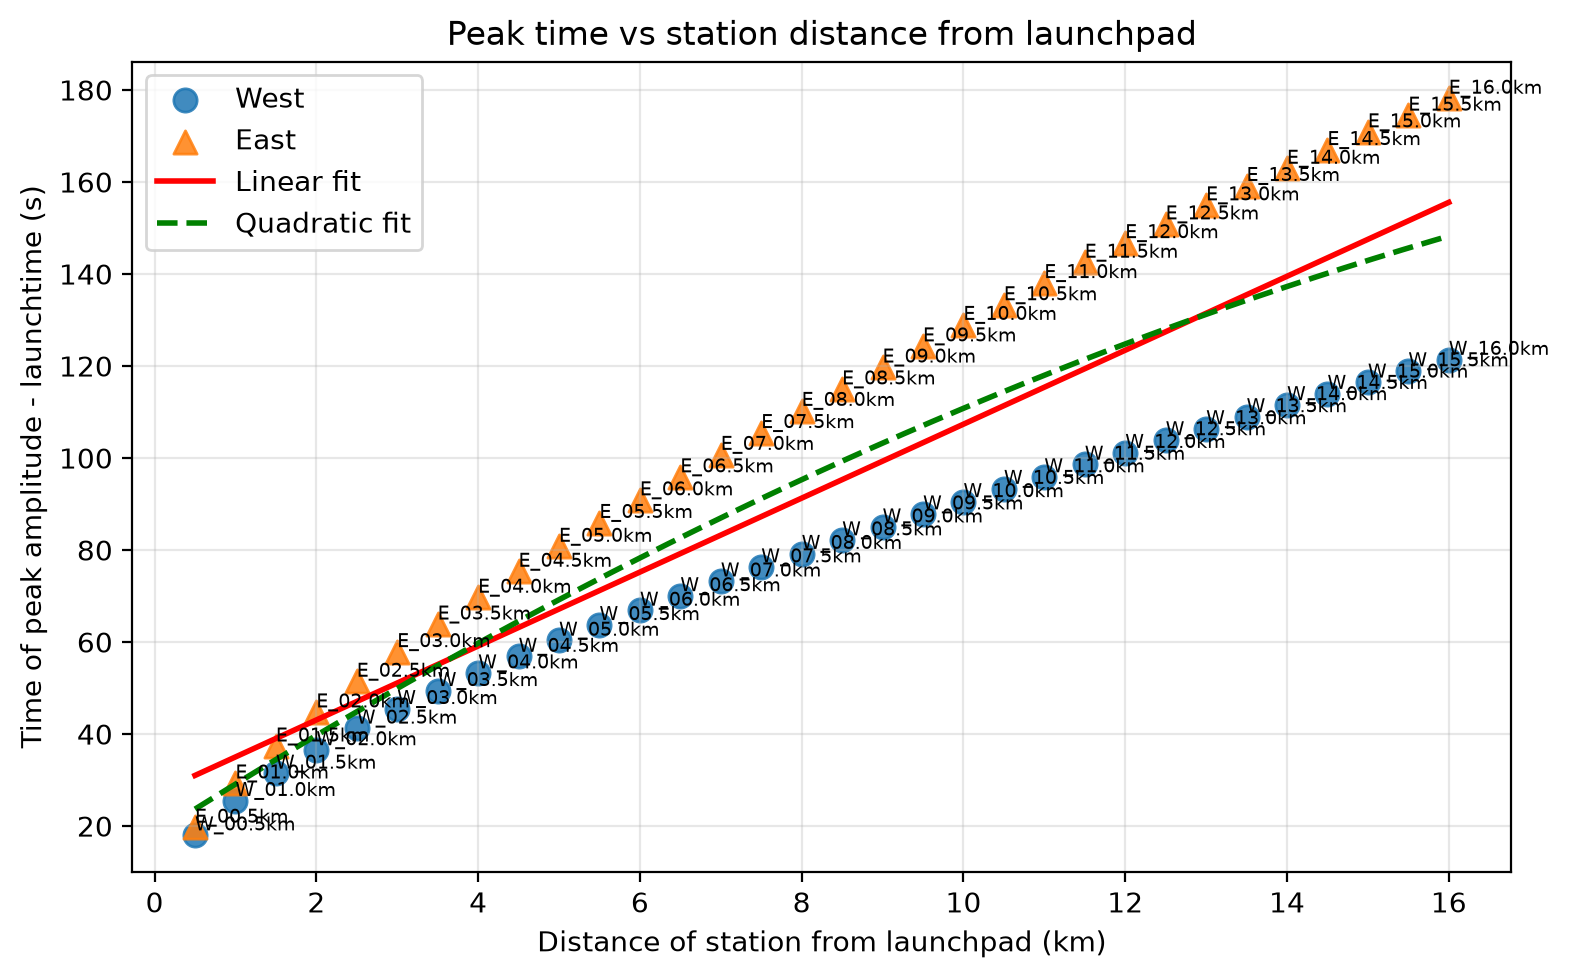
\includegraphics[width=0.8\textwidth]{synthetic_peaktime_vs_distance}
  \caption{Synthetic peak arrival time versus distance on the idealized lines
    for the originally assumed directivity [35]. Red: linear fit
    $t = 29.6 + 8.0\,r$~s ($r$ in km, apparent speed 125~m~s$^{-1}$); green
    dashed: quadratic fit.}
\end{figure}

\begin{figure}[p]
  \centering
  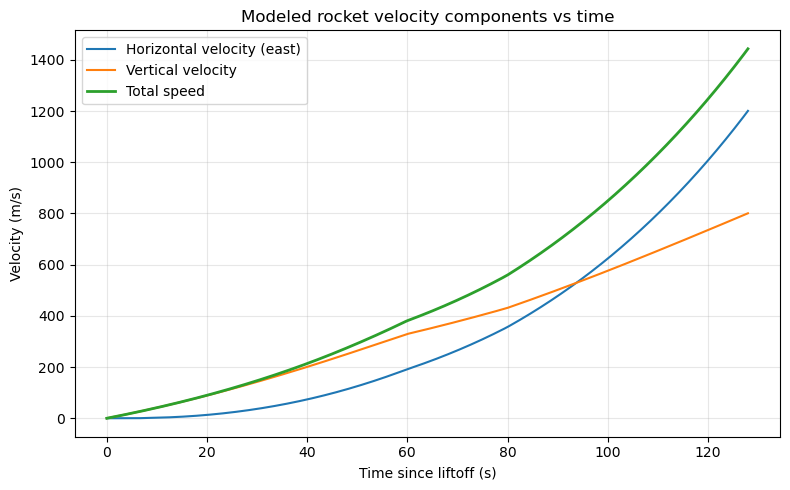
\includegraphics[width=0.85\textwidth]{velocity_vs_time}
  \caption{Modelled rocket velocity components and total speed versus time
    since liftoff [35].}
\end{figure}


\begin{table}[p]
  \centering
  \caption{Station locations and instrumentation, sorted by distance
    from SLC-39B. Gem 363, recorded under the provisional code
    \texttt{1R.UNK..HD1}, was 8~m from B20 according to its GPS log.}
  \label{tab:stations}
  \small
  \begin{tabular}{lrrrrl}
    \toprule
    Station & Lat ($^{\circ}$) & Lon ($^{\circ}$) & Distance (km) &
      Azimuth ($^{\circ}$) & Instrumentation \\
    \midrule
    B14  & 28.6322 & $-$80.6158 & 0.74 & 41.4  &
      Trillium/Centaur, infraBSU, Gem, SmartSolo \\
    B01  & 28.6214 & $-$80.6067 & 1.53 & 115.0 &
      Trillium/Centaur, infraBSU, Gem, SmartSolo \\
    B03  & 28.6428 & $-$80.6236 & 1.75 & 351.0 &
      Trillium/Centaur, infraBSU, Gem, SmartSolo \\
    B12  & 28.6217 & $-$80.6472 & 2.65 & 256.6 &
      G\"{u}ralp Certimus, Gem, SmartSolo \\
    B05  & 28.6400 & $-$80.6450 & 2.76 & 300.9 &
      Trillium/Centaur, infraBSU \\
    B07  & 28.6072 & $-$80.5942 & 3.42 & 130.4 &
      G\"{u}ralp Certimus, Gem (2), SmartSolo \\
    B24  & 28.5806 & $-$80.6408 & 5.53 & 200.7 &
      Trillium/Centaur, infraBSU, Gem (2), SmartSolo \\
    B23  & 28.5786 & $-$80.6078 & 5.54 & 166.7 &
      Silicon Audio accel., Gem, SmartSolo \\
    B24RE& 28.5812 & $-$80.6433 & 5.56 & 203.3 & Gem \\
    B29  & 28.6181 & $-$80.6769 & 5.58 & 259.5 &
      Trillium/Centaur, infraBSU, Gem (2), SmartSolo$^{a}$ \\
    B24LT& 28.5805 & $-$80.6429 & 5.61 & 202.6 & Gem \\
    B20W & 28.5737 & $-$80.5725 & 7.58 & 141.4 & Gem, SmartSolo \\
    B20  & 28.5736 & $-$80.5722 & 7.61 & 141.3 &
      Trillium/Centaur, infraBSU, Chaparral M25, Gem (3), SmartSolo \\
    B20S & 28.5733 & $-$80.5722 & 7.63 & 141.5 & Gem, SmartSolo \\
    \bottomrule
    \multicolumn{6}{l}{$^{a}$ No data during the launch.}
  \end{tabular}
\end{table}

\begin{table}[p]
  \centering
  \caption{Peak pressure ($>$0.5~Hz) and peak vertical ground velocity
    ($>$1~Hz) in the first 180~s after launch, over unclipped samples.
    $\geq$: overflowed Gem, value is the peak outside the overflow
    interval. $t_\text{pk}$: time of the peak after launch.
    $L_\text{pk}$: peak level, dB re \SI{20}{\micro\pascal}. B03's
    infraBSU (DD0) is omitted (hardware fault).}
  \label{tab:amplitudes}
  \scriptsize
  \begin{tabular}{lrrlrrrl}
    \toprule
    Channel & $r$ (km) & Az ($^{\circ}$) & Sensor & $p_\text{pk}$ (Pa) & $L_\text{pk}$ (dB) & $t_\text{pk}$ (s) & Note \\
    \midrule
    B14..HDF & 0.74 & 41 & Gem & $\geq$95 & 134 & 31.5 & overflow \\
    B14..HDI & 0.74 & 41 & Gem & $\geq$90 & 133 & 31.5 & overflow \\
    B01..HDI & 1.53 & 115 & Gem & $\geq$99 & 134 & 35.6 & overflow \\
    B01.00.DD0 & 1.53 & 115 & infraBSU & 512 & 148 & 22.0 &  \\
    B01.00.DD1 & 1.53 & 115 & infraBSU & 454 & 147 & 22.2 &  \\
    B01.00.DD2 & 1.53 & 115 & infraBSU & 434 & 147 & 23.2 &  \\
    B03..HDI & 1.75 & 351 & Gem & $\geq$128 & 136 & 5.6 & overflow \\
    B12..HDF & 2.65 & 257 & Gem & $\geq$98 & 134 & 38.0 & overflow \\
    B05.00.DD0 & 2.76 & 301 & infraBSU & 329 & 144 & 12.0 &  \\
    B07..HDF & 3.42 & 130 & Gem & 121 & 136 & 35.3 &  \\
    B07.10.HDF & 3.42 & 130 & Gem & $\geq$114 & 135 & 42.9 & overflow \\
    B24..HDI & 5.53 & 201 & Gem & 87 & 133 & 38.8 &  \\
    B24..HDF & 5.53 & 201 & Gem & 81 & 132 & 38.8 &  \\
    B23..HDF & 5.54 & 167 & Gem & 82 & 132 & 45.5 &  \\
    B24RE..HDF & 5.56 & 203 & Gem & 98 & 134 & 38.9 &  \\
    B29..HDF & 5.58 & 260 & Gem & 100 & 134 & 38.8 &  \\
    B29..HDI & 5.58 & 260 & Gem & 93 & 133 & 38.8 &  \\
    B29.00.DD0 & 5.58 & 260 & infraBSU & 121 & 136 & 38.7 &  \\
    B24LT..HDF & 5.61 & 203 & Gem & 105 & 134 & 39.0 &  \\
    B20W..HDF & 7.58 & 141 & Gem & 45 & 127 & 71.3 &  \\
    B20..HDF & 7.61 & 141 & Gem & 45 & 127 & 71.4 &  \\
    B20.10.HDI & 7.61 & 141 & Gem & 45 & 127 & 71.3 &  \\
    B20S..HDF & 7.63 & 141 & Gem & 42 & 126 & 71.5 &  \\
    \midrule
    Channel & $r$ (km) & Az ($^{\circ}$) & Sensor & $v_\text{pk}$ (mm~s$^{-1}$) & & $t_\text{pk}$ (s) & Note \\
    \midrule
    B14..DPZ & 0.74 & 41 & SmartSolo & 7.45 & & 4.9 &  \\
    B01..DPZ & 1.53 & 115 & SmartSolo & 2.98 & & 23.2 &  \\
    B01.00.DHZ & 1.53 & 115 & Trillium & 2.91 & & 23.2 &  \\
    B03..DPZ & 1.75 & 351 & SmartSolo & 2.50 & & 23.2 &  \\
    B03.00.DHZ & 1.75 & 351 & Trillium & 0.072 & & 23.3 & faulty \\
    B12..DPZ & 2.65 & 257 & SmartSolo & 2.57 & & 27.0 &  \\
    B05.00.DHZ & 2.76 & 301 & Trillium & 1.60 & & 24.5 & drift \\
    B07..DPZ & 3.42 & 130 & SmartSolo & 0.84 & & 49.0 &  \\
    B24..DPZ & 5.53 & 201 & SmartSolo & 0.92 & & 34.6 &  \\
    B23..DPZ & 5.54 & 167 & SmartSolo & 0.75 & & 48.5 &  \\
    B29.00.DHZ & 5.58 & 260 & Trillium & 0.99 & & 41.3 &  \\
    B20W..DPZ & 7.58 & 141 & SmartSolo & 0.57 & & 57.8 &  \\
    B20..DPZ & 7.61 & 141 & SmartSolo & 0.66 & & 56.5 &  \\
    B20S..DPZ & 7.63 & 141 & SmartSolo & 0.53 & & 59.4 &  \\
    \bottomrule
  \end{tabular}
\end{table}

\end{document}
